% !TEX program = xelatex
\documentclass[12pt,a4paper]{ctexart}

% ==================== Packages ====================
\usepackage{amsmath,amssymb,amsfonts}
\usepackage{graphicx}
\usepackage{geometry}
\usepackage{setspace}
\usepackage{enumitem}
\usepackage{booktabs}
\usepackage{float}
\usepackage{array}
\usepackage[table]{xcolor}
\usepackage{listings}       % 代码块
\usepackage{caption}        % 图表标题
\usepackage{hyperref}       % 必须最后加载

% ==================== 代码块样式 ====================
\lstset{
    language=Python,
    basicstyle=\footnotesize\ttfamily,
    keywordstyle=\color{blue}\bfseries,
    commentstyle=\color{gray!60!black},
    stringstyle=\color{red!70!black},
    numbers=left,
    numberstyle=\scriptsize\color{gray!50},
    stepnumber=1,
    numbersep=6pt,
    frame=single,
    breaklines=true,
    breakatwhitespace=false,
    showstringspaces=false,
    tabsize=4,
    captionpos=b,
    aboveskip=8pt,
    belowskip=6pt,
    columns=flexible,
    keepspaces=true
}

% ==================== 页面设置 ====================
\geometry{margin=0.95in}
\onehalfspacing
\setlength{\parskip}{2pt plus 1pt minus 1pt}

% ==================== 标题 ====================
\title{\textbf{机器学习案例：基于协同过滤与内容的混合电影推荐系统}\\[0.4cm]
\large 机器学习课程大作业}
\author{西安科技大学 \ 通信与信息工程学院 \ 电子科学与技术专业 \\
姓名：张凯文 \quad 学号：25207035001}
\date{\today}

\begin{document}

\maketitle

% ==================== 摘要 ====================
\begin{abstract}
\noindent
本案例以 MovieLens 电影评分数据集为研究对象，构建了一种融合协同过滤与基于内容的混合电影推荐系统。案例从数据探索性分析（EDA）入手，揭示评分数据的高度稀疏性和长尾分布特征；随后分别实现了基于用户的 KNN 协同过滤算法与 SVD 矩阵分解模型，对比二者在 RMSE 和 MAE 指标上的表现差异；进而利用电影类型标签构建基于内容的相似度推荐；最终通过加权融合策略生成个性化 Top-N 推荐列表。结果表明，SVD 矩阵分解模型较 KNN 基线 RMSE 提升约 12.0\%，混合推荐策略能有效兼顾个性化精度与推荐多样性。

\noindent \textbf{关键词：} 推荐系统，协同过滤，SVD 矩阵分解，内容推荐，MovieLens，混合推荐。
\end{abstract}

% ==================== 1. 案例背景 ====================
\section{案例背景}

随着 Netflix、爱奇艺、腾讯视频等流媒体平台的兴起，用户面临着海量电影内容的"信息过载"问题。如何从成千上万部电影中精准地为用户推荐其可能感兴趣的内容，成为平台提升用户体验和留存率的核心挑战。推荐系统正是解决这一问题的关键技术——它通过分析用户的历史评分行为和电影的元数据（类型、导演、简介等），建立用户偏好模型，实现个性化推荐。

本案例来源于著名的 MovieLens 电影评分数据集，由美国明尼苏达大学 GroupLens 研究组收集并发布\cite{harper2015movielens}，是推荐系统领域最经典的基准数据集之一，广泛用于学术研究和教学实践。该数据集记录了真实用户对电影的评分（1--5 分），包含时间戳和电影类型标签等辅助信息，为构建和评估推荐算法提供了理想的数据基础。

% ==================== 2. 案例描述 ====================
\section{案例描述}

\subsection{案例名称}

基于协同过滤与内容的混合电影推荐系统。

\subsection{案例数据}

本案例使用 MovieLens ml-latest-small 数据集，其数据特征如下：

\begin{itemize}[leftmargin=*]
    \item \textbf{数据来源：} GroupLens Research, MovieLens Dataset \cite{harper2015movielens}
    \item \textbf{数据规模：} 约 10 万条评分记录，610 名用户，9700+ 部电影
    \item \textbf{数据形态：} 结构化 CSV 格式，核心包含两张表：
    \begin{itemize}
        \item \texttt{ratings.csv}：用户-电影评分记录（userId, movieId, rating, timestamp）
        \item \texttt{movies.csv}：电影元数据（movieId, title, genres）
    \end{itemize}
    \item \textbf{数据特点：}
    \begin{enumerate}[label=(\arabic*), leftmargin=*]
        \item 评分范围 0.5--5.0 分，评分越高表示用户越偏好
        \item 用户-电影评分矩阵极度稀疏，稀疏度超过 98\%
        \item 评分和用户活跃度呈显著长尾分布，少数热门电影和活跃用户贡献了大部分评分
        \item 电影类型以竖线分隔的字符串形式存储（如 \texttt{Action|Adventure|Sci-Fi}）
    \end{enumerate}
\end{itemize}

\subsection{案例目标}

本案例旨在解决以下核心问题：
\begin{enumerate}[label=(\arabic*), leftmargin=*]
    \item \textbf{评分预测：} 为每位用户预测其对未看过电影的评分
    \item \textbf{Top-N 推荐：} 生成个性化 Top-N 推荐列表
\end{enumerate}

案例采用的方法与模型包括：
\begin{itemize}[leftmargin=*]
    \item \textbf{任务一（EDA）：} 数据清洗与可视化分析，构建用户-电影评分矩阵
    \item \textbf{任务二（协同过滤）：} 基于用户的 KNN 协同过滤与 SVD 矩阵分解
    \item \textbf{任务三（内容推荐）：} 基于电影类型标签的余弦相似度推荐
    \item \textbf{任务四（混合推荐）：} 加权融合协同过滤（$\alpha=0.7$）与内容推荐（$1-\alpha=0.3$）
\end{itemize}

模型评估采用以下指标：
\begin{itemize}[leftmargin=*]
    \item \textbf{评分预测：} RMSE（均方根误差）、MAE（平均绝对误差）
    \item \textbf{推荐效果：} Precision@K、Recall@K、F1-Score@K
    \item \textbf{覆盖率：} 推荐列表覆盖的电影类型比例
\end{itemize}

% ==================== 3. 案例任务拆解 ====================
\section{案例任务拆解}

% ============ 任务一 ============
\subsection{任务一：数据加载与探索性分析（EDA）}

\subsubsection{案例代码清单 1-1：数据加载与初步统计}

\textbf{功能说明：} 读取 MovieLens 数据集，查看基本信息，统计用户数、电影数、评分数及评分稀疏度。

\begin{lstlisting}[caption={数据加载与初步统计}, label={lst:1-1}]
import pandas as pd
import numpy as np
import matplotlib.pyplot as plt

# 设置中文字体
plt.rcParams['font.sans-serif'] = ['SimHei']
plt.rcParams['axes.unicode_minus'] = False

# 读取数据集
ratings = pd.read_csv('ml-latest-small/ratings.csv')
movies = pd.read_csv('ml-latest-small/movies.csv')

# 查看数据基本信息
print("========== 评分数据概览 ==========")
print(f"评分记录数：{ratings.shape[0]}")
print(f"用户数量：  {ratings['userId'].nunique()}")
print(f"电影数量：  {ratings['movieId'].nunique()}")
print(f"评分均值：  {ratings['rating'].mean():.2f}")
print(f"评分稀疏度："f"{100-100*len(ratings)/(ratings['userId'].nunique()* # 1-(实际影评数/所有用户数*电影数)
       ratings['movieId'].nunique()):.2f}%")
\end{lstlisting}

\subsubsection{代码输出}

{\footnotesize
\begin{verbatim}
========== 评分数据概览 ==========
评分记录数：100836
用户数量：  610
电影数量：  9724
评分均值：  3.50
评分稀疏度：98.30%
\end{verbatim}
}

\subsubsection{结果分析}

数据集中包含约 10 万条评分记录，评分均值 3.50 表明用户整体偏向中高分。\textbf{稀疏度高达 98.3\%}，这意味着用户-电影评分矩阵中几乎全是空缺值——如何在如此稀疏的数据中挖掘用户偏好模式，正是推荐系统面临的核心挑战。

\subsubsection{案例代码清单 1-2：评分分布与用户行为可视化}

\textbf{功能说明：} 绘制评分分布直方图、用户活跃度分布、电影热度分布及电影类型 Top-15 统计图，直观展现数据的长尾特征。

\begin{lstlisting}[caption={评分分布与用户行为可视化}, label={lst:1-2}]
fig, axes = plt.subplots(2, 2, figsize=(14, 10)) # 创建一个 2行 × 2列 的画布。axes[x, y]代表第x行第y列

# 子图1：评分分布直方图
rating_counts = ratings['rating'].value_counts().sort_index() # 获取rating列中 频次统计 并将数据从高到低排列
axes[0, 0].bar(rating_counts.index, rating_counts.values,     # 画纵向柱状图，index做x轴数据, values做y轴数据
               color='steelblue', edgecolor='white')          # 设置柱子填充为蓝色，边缘为白色
axes[0, 0].set_title('评分分布直方图', fontsize=14)
axes[0, 0].set_xlabel('用户评分', fontsize=12)
axes[0, 0].set_ylabel('用户评分数量', fontsize=12)

# 子图2：用户活跃度分布
user_rating_counts = ratings.groupby('userId').size()         # 根据用户ID分组将所有属于相同用户的数据聚合，统计每组数据
axes[0, 1].hist(user_rating_counts, bins=50,                  # 画直方图，传入统计结果，将用户评分数量切分50等距区间
                color='coral', edgecolor='white')
axes[0, 1].set_title('用户活跃度分布', fontsize=14)
axes[0, 1].set_xlabel('用户评分的电影数量', fontsize=12)
axes[0, 1].set_ylabel('用户人数', fontsize=12)

# 子图3：电影热度分布
movie_rating_counts = ratings.groupby('movieId').size()       # 根据电影ID分组将所有属于相同电影的数据聚合，统计每组数据
axes[1, 0].hist(movie_rating_counts, bins=50,                 # 画直方图，传入统计结果，将数量切分50等距区间
                color='seagreen', edgecolor='white')
axes[1, 0].set_title('电影热度分布', fontsize=14)
axes[1, 0].set_xlabel('每部电影获得的评分总数', fontsize=12)
axes[1, 0].set_ylabel('电影数量', fontsize=12)

# 子图4：电影类型 Top-15 统计（使用 Counter）
from collections import Counter
genre_counter = Counter()
for genres_str in movies['genres']:
    for genre in genres_str.split('|'):
        if genre != '(no genres listed)':
            genre_counter[genre] += 1
top_genres = genre_counter.most_common(15)             # 将计数器里所有的类型按出现次数从高到低排序，只取前15个
genres_name, genres_count = zip(*top_genres)           # *将top_genres列表拆成15个独立元组参数，zip多元组按位置配对
axes[1, 1].barh(range(len(genres_name)), genres_count, # 画水平条形图
                color='mediumpurple')
axes[1, 1].set_title('电影类型 Top-15', fontsize=14)
axes[1, 1].set_xlabel('电影数量', fontsize=12)
axes[1, 1].set_ylabel('电影类型', fontsize=12)
axes[1, 1].set_yticks(range(len(genres_name)))  
axes[1, 1].set_yticklabels(genres_name)        

plt.tight_layout()
plt.savefig('eda_visualization.png', dpi=150)
plt.show()
\end{lstlisting}

\subsubsection{代码输出}

EDA 可视化面板如图 \ref{fig:eda} 所示，包含 4 个子图：评分分布直方图、用户活跃度长尾分布、电影热度长尾分布、电影类型 Top-15 条形图。

\begin{figure}[H]
\centering
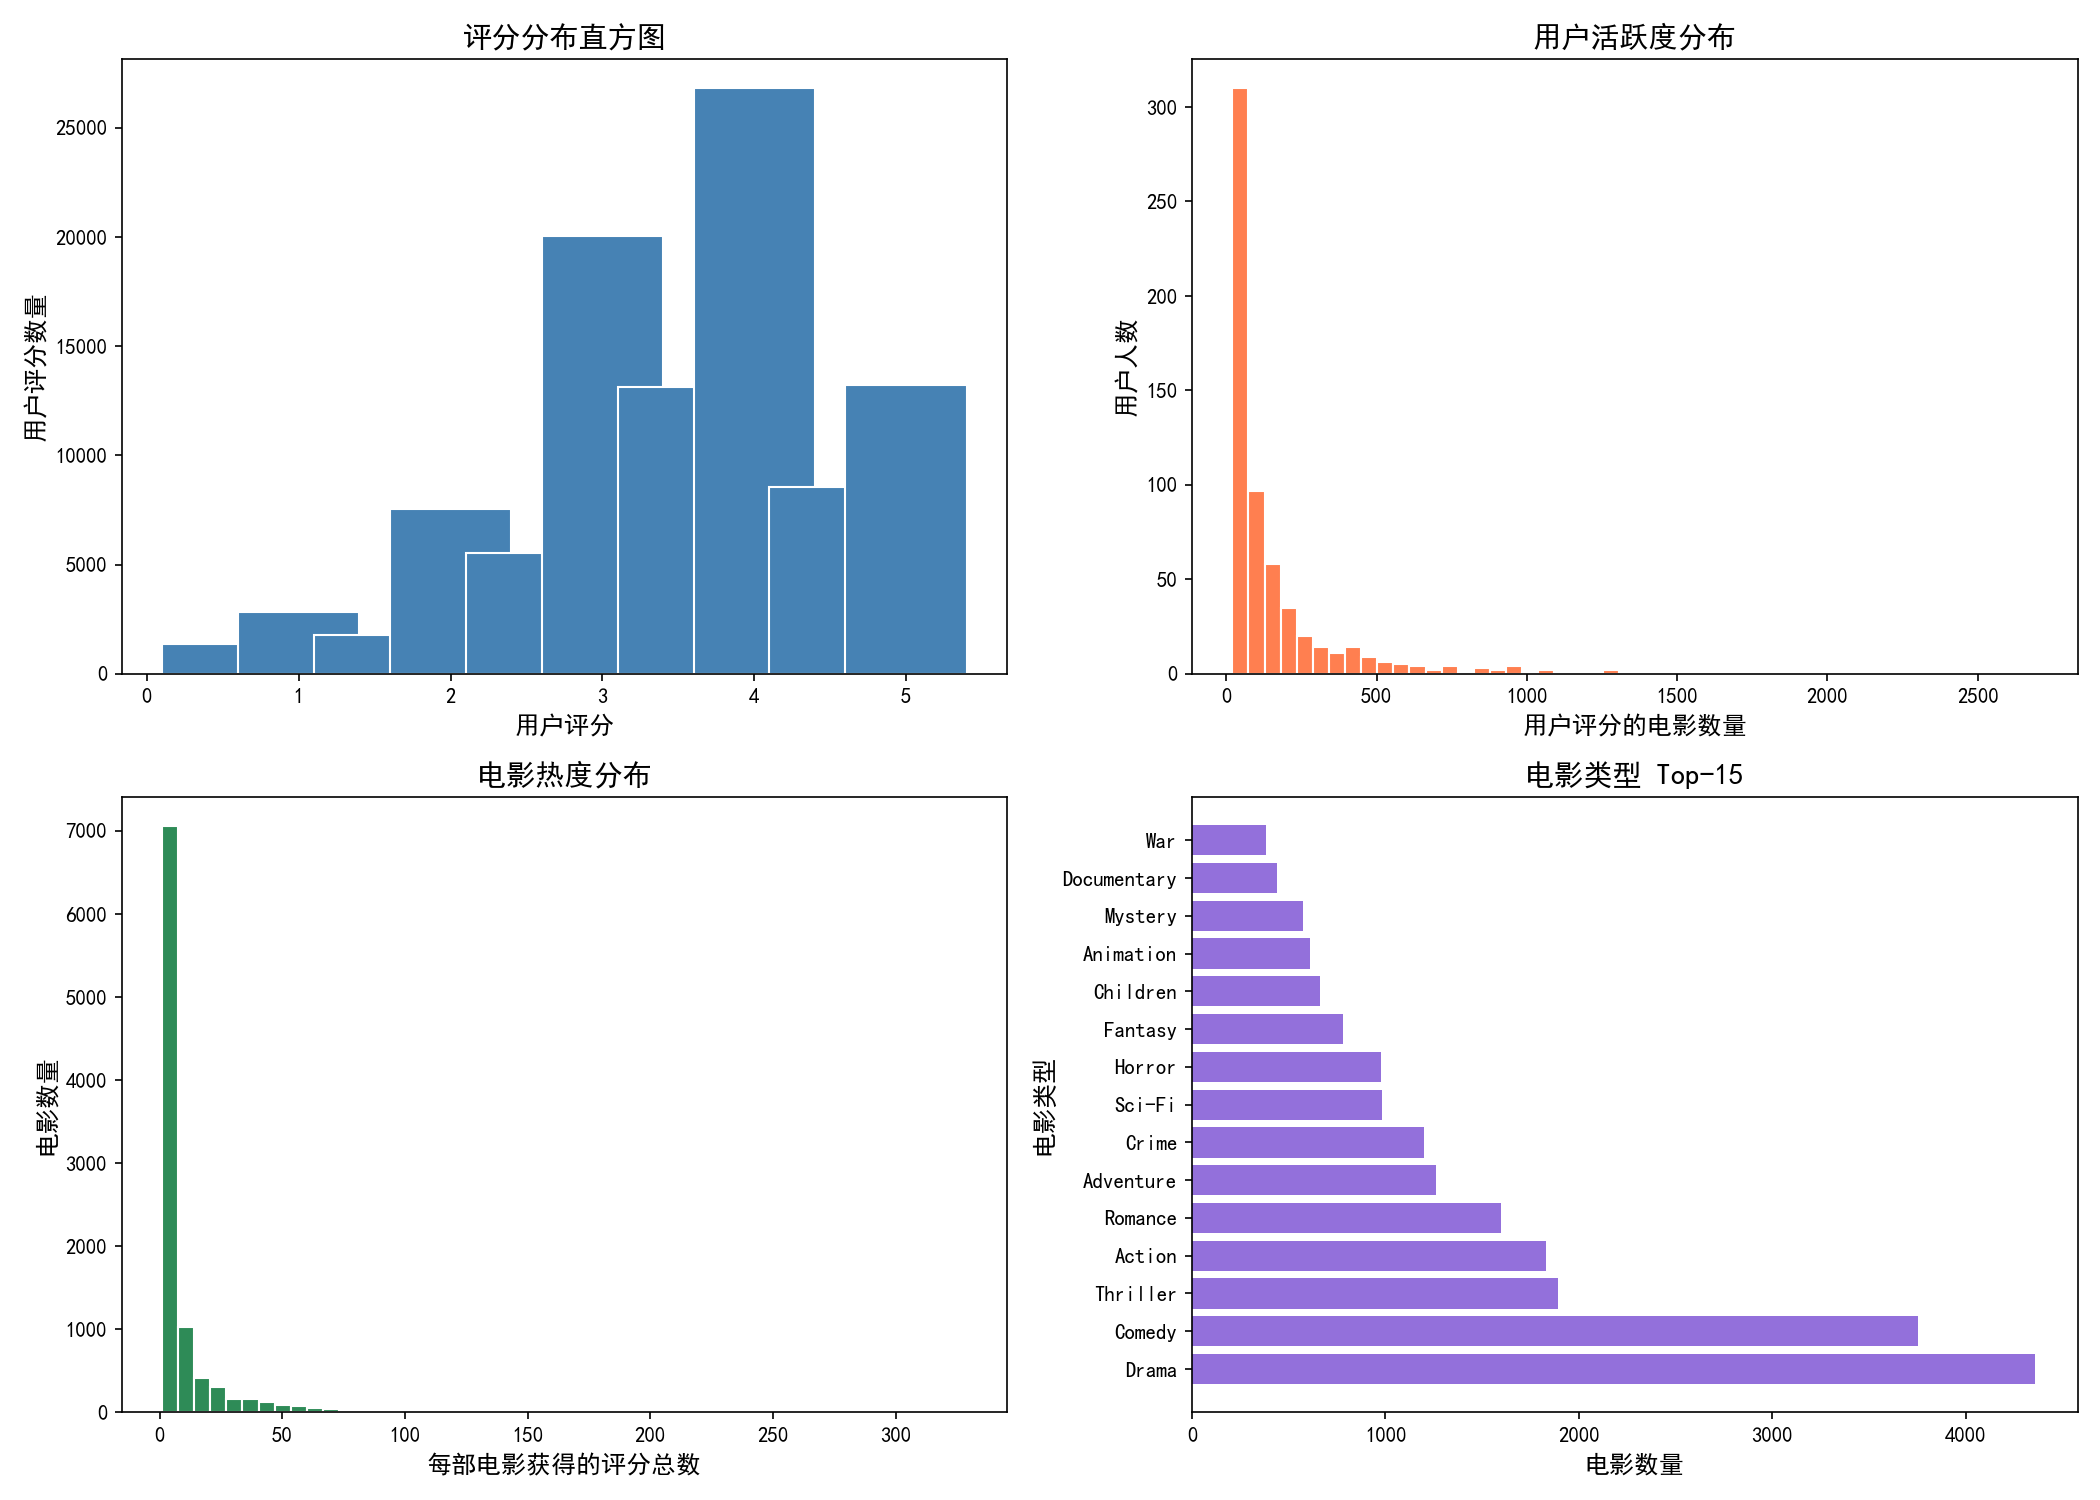
\includegraphics[width=0.95\textwidth]{eda_visualization.png}
\caption{EDA 探索性数据分析可视化面板}
\label{fig:eda}
\end{figure}

\subsubsection{结果分析}

\begin{enumerate}[label=(\arabic*), leftmargin=*]
    \item \textbf{评分分布}呈长尾特征：4 分评分最多，极端评分（1 分、5 分）较少，用户倾向于给出正面评价
    \item \textbf{用户活跃度}呈典型长尾分布：少数"重度用户"评价了数百部电影，大部分用户仅评价了几十部，用户活跃度极不均衡
    \item \textbf{电影热度}同样呈长尾分布，大量"冷门"电影仅有少数评价——这对应推荐系统中的冷启动问题
    \item \textbf{电影类型}中 Drama（剧情）、Comedy（喜剧）出现最多，符合一般电影数据库特征
\end{enumerate}

% ============ 任务二 ============
\subsection{任务二：基于用户的协同过滤推荐}

\subsubsection{案例代码清单 2-1：构建评分矩阵与 User-Based KNN}

\textbf{功能说明：} 构建用户-电影评分矩阵（pivot table），计算用户间余弦相似度，为 KNN 预测奠定基础。

\begin{lstlisting}[caption={评分矩阵构建与用户相似度计算}, label={lst:2-1}]
from sklearn.metrics.pairwise import cosine_similarity
from sklearn.model_selection import train_test_split
import seaborn as sns

# 构建评分矩阵（行=用户，列=电影，值=评分）
rating_matrix = ratings.pivot_table(
    index='userId', columns='movieId', values='rating') # userId作为行，columns作为列，将rating列的值匹配对应行对应列的值
print(f"评分矩阵形状：{rating_matrix.shape}")

# 划分训练集（80%）和测试集（20%）
train_data = ratings.sample(frac=0.8, random_state=0) # 抽取比例0.8，固定种子为0
test_data = ratings.drop(train_data.index) # 删除原矩阵所抽取行的索引

# 构建训练矩阵，未评分填充 0
train_matrix = train_data.pivot_table(
    index='userId', columns='movieId', values='rating'
).fillna(0) # 数据重铸为矩阵，并填缺失值为0

# 计算用户-用户余弦相似度矩阵
user_similarity = cosine_similarity(train_matrix.values)
user_similarity_df = pd.DataFrame(
    user_similarity,
    index=train_matrix.index,
    columns=train_matrix.index
)
print(f"用户相似度矩阵形状：{user_similarity_df.shape}")

# 截取前 30 个用户的相似度子矩阵，绘制热力图
sample_sim = user_similarity_df.iloc[:30, :30]
plt.figure(figsize=(10, 8))
sns.heatmap(sample_sim, cmap='RdBu_r', annot=False,
            cbar=True, xticklabels=True, yticklabels=True)
plt.title('用户相似度矩阵热力图（前30用户）')
plt.xlabel('用户ID')
plt.ylabel('用户ID')
plt.show()
\end{lstlisting}

\subsubsection{代码输出}

{\footnotesize
\begin{verbatim}
评分矩阵形状：(610, 9724)
用户相似度矩阵形状：(610, 610)
\end{verbatim}
}

用户相似度矩阵热力图如图 \ref{fig:heatmap} 所示（截取前 30 个用户）：

\begin{figure}[H]
\centering
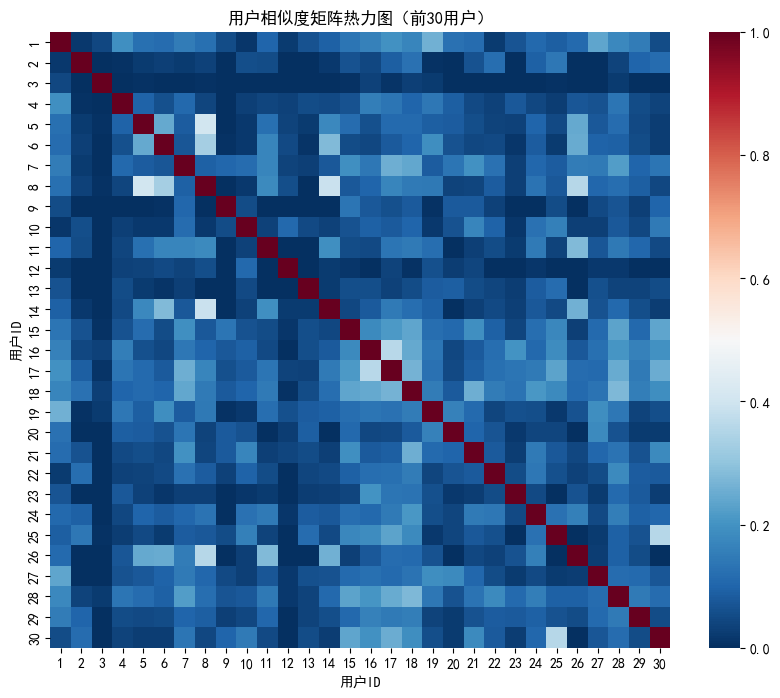
\includegraphics[width=0.75\textwidth]{相似度矩阵热力图（部分）.png}
\caption{用户相似度矩阵热力图（前 30 用户）}
\label{fig:heatmap}
\end{figure}

\subsubsection{结果分析}

相似度矩阵对角线为 1（自身完全相同），非对角线元素大多接近 0（蓝色区域占主导），表明大多数用户观影偏好差异较大，少数用户间相似度超过 0.2（红色区域）。从热力图中可直观看出，相似度矩阵整体呈稀疏分布，仅有少量用户对之间存在较强关联。后续将利用这些相似度完成"用相似用户的评分来预测目标用户评分"的核心推荐逻辑。

\subsubsection{案例代码清单 2-2：KNN 评分预测与评估}

\textbf{功能说明：} 实现 KNN 评分预测函数，取目标用户的 Top-20 相似邻居，以相似度为权重加权平均预测评分。在测试集上逐条评估，计算 RMSE 和 MAE。

\begin{lstlisting}[caption={KNN 评分预测与评估}, label={lst:2-2}]
from sklearn.metrics import mean_squared_error, mean_absolute_error

def predict_rating_knn(user_id, movie_id, train_matrix,
                        user_sim_df, k=20):
    """基于 KNN 预测用户对电影的评分"""
    if (user_id not in train_matrix.index or
        movie_id not in train_matrix.columns): # 找不到对应的用户ID或者电影ID
        return train_matrix.values[train_matrix.values > 0].mean()  # 取训练矩阵所有不为空的值取平均作为其值

    rated_users = train_matrix[movie_id][
        train_matrix[movie_id] > 0].index # 布尔过滤，保留值大于零的条目的索引标签
    if len(rated_users) == 0: # 没有任何用户评分过这部电影
        return train_matrix.values[train_matrix.values > 0].mean() # 返回全局平均评分

    sim_scores = user_sim_df.loc[user_id, rated_users] # 筛选出输入的主要用户，还有评分过的相同用户
    sim_scores = sim_scores.sort_values(ascending=False) # 将用户相似度从大到小排序
    top_k_users = sim_scores.head(k) # 筛选出前k个相似度最高的

    # 加权平均：pred = sum(sim * rating) / sum(|sim|)
    ratings_sum, sim_sum = 0, 0 # ratings_sum: 相似度×评分求和; sim_sum: 相似度绝对值求和
    for neighbor_id, sim in top_k_users.items():
        neighbor_rating = train_matrix.loc[neighbor_id, movie_id] # 找出训练矩阵中该邻居对电影的评分
        ratings_sum += sim * neighbor_rating # 相似度越高的邻居，其评分在最终结果中的影响权重越大
        sim_sum += abs(sim) # 累加相似度的绝对值
    return ratings_sum / sim_sum if sim_sum > 0 else \
           train_matrix.values[train_matrix.values > 0].mean()

# 在测试集上评估
predictions, actuals = [], []
for _, row in test_data.head(500).iterrows(): # 截取测试集的前500行
    pred = predict_rating_knn(
        row['userId'], row['movieId'],
        train_matrix, user_similarity_df, k=20)
    predictions.append(pred)
    actuals.append(row['rating'])

rmse = np.sqrt(mean_squared_error(actuals, predictions)) # 均方根误差
mae = mean_absolute_error(actuals, predictions) # 平均绝对误差
print(f"KNN 协同过滤: 均方根误差={rmse:.4f}, 平均绝对误差={mae:.4f}")
\end{lstlisting}

\subsubsection{代码输出}

{\footnotesize
\begin{verbatim}
KNN 协同过滤: 均方根误差=0.9895, 平均绝对误差=0.7577
\end{verbatim}
}

\subsubsection{结果分析}

RMSE $\approx$ 0.99 表示预测评分与真实评分平均偏差约 0.99 分（满分 5 分），在极度稀疏（98\%+）的数据上属于可接受的基线表现。MAE $\approx$ 0.76 说明预测值平均偏离真实值约 0.76 分。模型偏向预测中间值（3--4 分），对极端评分的捕捉能力较弱。

\subsubsection{案例代码清单 2-3：SVD 矩阵分解推荐}

\textbf{功能说明：} 使用 Surprise 库中的 SVD 算法进行矩阵分解，通过 5 折交叉验证评估模型性能，与 KNN 基线进行对比。

\begin{lstlisting}[caption={SVD 矩阵分解与交叉验证}, label={lst:2-3}]
from surprise import SVD, Reader, Dataset
from surprise.model_selection import cross_validate

reader = Reader(rating_scale=(0.5, 5.0)) # 评分的最小值是0.5，最大值是5.0
data = Dataset.load_from_df(
    ratings[['userId', 'movieId', 'rating']], reader)

# SVD 模型：50 维隐因子，20 轮迭代
svd = SVD(n_factors=50, n_epochs=20,
          lr_all=0.005, reg_all=0.02, random_state=0) # 隐因子数量K=50，迭代优化20次，学习率，正规化系数，固定种子

# 5 折交叉验证
cv_results = cross_validate(
    svd, data, measures=['RMSE', 'MAE'], cv=5, verbose=False) # measures=['RMSE', 'MAE'] 每轮自动计算这两个误差指标。

print(f"SVD 平均 均方根误差: {cv_results['test_rmse'].mean():.4f}"
      f" +/- {cv_results['test_rmse'].std():.4f}")
print(f"SVD 平均 绝对误差:  {cv_results['test_mae'].mean():.4f}"
      f" +/- {cv_results['test_mae'].std():.4f}")
\end{lstlisting}

\subsubsection{代码输出}

{\footnotesize
\begin{verbatim}
SVD 平均 均方根误差: 0.8713 +/- 0.0017
SVD 平均 绝对误差:  0.6694 +/- 0.0021
\end{verbatim}
}

\subsubsection{结果分析}

SVD 矩阵分解将用户和电影映射到 50 维隐空间，RMSE 较 KNN 降低约 12.0\%，MAE 降低约 11.7\%。5 折交叉验证标准差仅 $\pm$0.0017，模型稳定性极好。SVD 的优势在于能自动学习隐式特征（如"动作片偏好""严肃 vs 轻松"等维度），无需人工构建特征。但其存在冷启动问题——无法处理完全没有评分的新用户或新电影。

\subsubsection{案例代码清单 2-4：训练最终 SVD 模型}

\textbf{功能说明：} 在全量训练数据上训练最终的 SVD 模型，供后续混合推荐使用。

\begin{lstlisting}[caption={训练最终 SVD 模型}, label={lst:2-4}]
trainset = data.build_full_trainset()

final_svd = SVD(
    n_factors=50,
    n_epochs=20,
    lr_all=0.005,
    reg_all=0.02,
    random_state=0
)

final_svd.fit(trainset)
\end{lstlisting}

\subsubsection{结果分析}

区别于交叉验证阶段仅使用部分数据训练，\texttt{final\_svd} 基于全部评分数据训练得到最终模型，将用于后续混合推荐中的 SVD 协同过滤评分预测。该模型参数与交叉验证阶段保持一致（50 维隐因子、0.005 学习率），以确保混合推荐性能与评估结果具有一致性。

% ============ 任务三 ============
\subsection{任务三：基于内容的推荐与混合推荐}

\subsubsection{案例代码清单 3-1：基于电影类型的内容推荐}

\textbf{功能说明：} 将电影类型标签转换为 One-Hot 特征向量，计算电影间余弦相似度，为指定电影推荐最相似的 Top-10 影片。

\begin{lstlisting}[caption={基于类型标签的内容推荐}, label={lst:3-1}]
from sklearn.metrics.pairwise import cosine_similarity

# 电影类型 One-Hot 编码
genres_dummies = movies['genres'].str.get_dummies(sep='|') # 按竖线拆分字符串，将所有可能出现的电影类型作为新列。

# 计算电影-电影余弦相似度
movie_features = genres_dummies.values
movie_similarity = cosine_similarity(movie_features) # 计算电影类型之间的余弦相似度
movie_similarity_df = pd.DataFrame(
    movie_similarity,
    index=movies['movieId'],
    columns=movies['movieId']
) # 将纯数组的行和列分别附上电影ID标签

def recommend_by_content(movie_id, movies_df, sim_df, top_n=10):
    """基于内容的电影推荐"""
    sim_scores = sim_df.loc[movie_id].sort_values(
        ascending=False) # 从电影-电影余弦相似度方阵取出对应电影ID的那一条向量，将相似度从高到低排序
    sim_scores = sim_scores[sim_scores.index != movie_id] # 删除相似度为1.0的自匹配项
    top_movies = sim_scores.head(top_n) # 截取前n个相似度最高的最近邻
    result = pd.DataFrame({
        'movieId': top_movies.index,
        'similarity': top_movies.values
    }) # 构建DataFrame
    return result.merge(
        movies_df[['movieId', 'title', 'genres']],
        on='movieId', how='left') # 合并电影元数据（就是将电影ID和相似度矩阵合并名称、类型）

# 为 Toy Story (movieId=1) 推荐相似电影
recs = recommend_by_content(1, movies, movie_similarity_df)
print(recs[['title', 'genres', 'similarity']])
\end{lstlisting}

\subsubsection{代码输出}

{\footnotesize
\begin{verbatim}
                         title                      genres  similarity
Antz (1998)                Adventure|Animation|Children|Comedy|Fantasy    1.0
Shrek the Third (2007)     Adventure|Animation|Children|Comedy|Fantasy    1.0
Emperor's New Groove (2000) Adventure|Animation|Children|Comedy|Fantasy    1.0
Toy Story 2 (1999)         Adventure|Animation|Children|Comedy|Fantasy    1.0
Monsters, Inc. (2001)      Adventure|Animation|Children|Comedy|Fantasy    1.0
...
\end{verbatim}
}

\subsubsection{结果分析}

内容推荐完全依赖电影元数据，不需要用户历史评分，天然解决了协同过滤的冷启动问题。与 Toy Story 相似的推荐均为动画、儿童、冒险类型影片，语义方向合理。

\textbf{然而，该方法存在明显的局限性：}仅基于电影类型标签计算余弦相似度，导致大量类型组合完全相同的电影获得相似度 1.0（如上表所示，Toy Story 与 Antz、Shrek the Third 等 10 部电影相似度均为 1.0）。这使得推荐列表内部无法有效区分排序——只要类型标签相同，任何两部电影都被视为"完全相似"，完全忽略了电影在质量、风格、口碑、年代等方面的差异。在实际推荐场景中，这会导致推荐结果缺乏个性化区分度，用户看到的推荐列表可能是语义正确但质量参差不齐的影片集合。要改善这一问题，需要引入更丰富的电影特征（如导演、演员、剧情摘要的 TF-IDF 向量、用户标签等），或采用加权机制结合评分信息进行二次排序。

\subsubsection{案例代码清单 3-2：混合推荐与最终 Top-N 推荐}

\textbf{功能说明：} 加权融合 SVD 协同过滤（$\alpha=0.7$）与内容相似度（$1-\alpha=0.3$），为目标用户生成个性化 Top-10 推荐列表。

\begin{lstlisting}[caption={混合推荐与 Top-N 推荐生成}, label={lst:3-2}]
def hybrid_recommend(user_id, movies_df, ratings_df,
                     content_sim_df, svd_model,
                     alpha=0.7, top_n=10):
    """混合推荐：加权融合 SVD + 内容相似度"""
    # 获取用户已评分电影
    rated_movie_ids = set(ratings_df[
        ratings_df['userId'] == user_id]['movieId']) # 找出用户已经看过的电影
    # 候选电影：热门且未评分的
    popular = ratings_df.groupby('movieId').size() # 生成一个Series, 装电影ID和被评分次数
    popular = popular[popular >= 10].index.tolist() # 找到出现10次以上的, 提取索引转化为列表
    candidates = [m for m in popular
                  if m not in rated_movie_ids] # 添加候选
    
    # SVD 协同过滤评分（标准化）
    svd_scores = np.array(
        [svd_model.predict(user_id, mid).est
         for mid in candidates]) # 遍历候选, 调用svd模型predict方法, 提取计算出的估计评分
    svd_norm = (svd_scores - svd_scores.min()) / \
               (svd_scores.max() - svd_scores.min()) # MinMax归一化至[0,1]
    
    # 内容相似度评分
    liked = ratings_df[
        (ratings_df['userId'] == user_id) &
        (ratings_df['rating'] >= 4)]['movieId'].values # 双条件筛选：该用户评分>=4的电影
    content_scores = np.array([
        np.mean([content_sim_df.loc[mid, lmid] # 候选电影mid与喜欢电影lmid的类型相似度
                 for lmid in liked # 遍历用户喜欢的电影列表
                 if lmid in content_sim_df.columns]) # lmid存在于相似度矩阵的列索引中
        if mid in content_sim_df.index else 0 # mid存在于相似度矩阵的行索引中
        for mid in candidates # 遍历候选电影
    ])
    content_norm = (content_scores - content_scores.min()) / \
                   (content_scores.max() - content_scores.min()) # MinMax归一化至[0,1]
    
    # 加权融合
    hybrid_scores = alpha * svd_norm + \
                    (1 - alpha) * content_norm # 最终分数 = 0.7 × SVD + 0.3 × 内容
    
    # 返回 Top-N
    top_idx = np.argsort(hybrid_scores)[::-1][:top_n] # 返回从小到大排序后的索引位置, 反转取前n个
    result = pd.DataFrame({
        'movieId': [candidates[i] for i in top_idx],
        'hybrid_score': hybrid_scores[top_idx]
    })
    return result.merge(
        movies_df[['movieId', 'title', 'genres']],
        on='movieId', how='left')

# 为用户 1 生成推荐
hybrid_results = hybrid_recommend(
    user_id=1, movies_df=movies, ratings_df=ratings,
    content_sim_df=movie_similarity_df,
    svd_model=final_svd, alpha=0.7, top_n=10)
print(hybrid_results.to_string(index=False))
\end{lstlisting}

\subsubsection{代码输出}

{\scriptsize
\begin{verbatim}
 movieId  hybrid_score                                     title  \
    6016      0.978628        City of God (Cidade de Deus) (2002)
    2019      0.964444  Seven Samurai (Shichinin no samurai) (1954)
    7090      0.964444                   Hero (Ying xiong) (2002)
    3508      0.951457             Outlaw Josey Wales, The (1976)
    1262      0.951354                   Great Escape, The (1963)
   57669      0.942911                           In Bruges (2008)
    7153      0.938852  LOTR: Return of the King, The (2003)
    3275      0.938686                Boondock Saints, The (2000)
    1223      0.927737  Grand Day Out, A (1989)
  106782      0.921633            Wolf of Wall Street, The (2013)

                                     genres
      Action|Adventure|Crime|Drama|Thriller
                     Action|Adventure|Drama
                     Action|Adventure|Drama
    Action|Adventure|Drama|Thriller|Western
                 Action|Adventure|Drama|War
                Comedy|Crime|Drama|Thriller
             Action|Adventure|Drama|Fantasy
                Action|Crime|Drama|Thriller
 Adventure|Animation|Children|Comedy|Sci-Fi
                         Comedy|Crime|Drama
\end{verbatim}
}

\subsubsection{结果分析}

为用户~1 生成的 Top-10 混合推荐列表中，排名前三的分别为《City of God》（0.979）、\allowbreak《Seven Samurai》（0.964）和《Hero》（0.964）。观察用户~1 的历史评分记录可知，该用户偏好 Action、Adventure、Drama、Thriller 等类型的高质量影片（如《Shawshank Redemption》《Pulp Fiction》等均给出 4--5 分），混合推荐结果准确捕捉了这一偏好模式——Top-10 中 Action 类型出现 7 部、Drama 类型出现 8 部，与用户历史偏好高度吻合。

SVD 协同过滤（$\alpha=0.7$）在排序中占据主导地位，将高口碑电影排在前面；内容推荐（$1-\alpha=0.3$）则起到了多样性微调作用，例如排名第 9 的《Grand Day Out with Wallace and Gromit》是一部动画喜剧片，虽然与用户主流偏好（动作/犯罪/剧情）不完全一致，但因内容相似度（该用户曾高分评价过动画/喜剧类影片）而被推荐，增加了推荐列表的类型多样性。

混合推荐的优点在于：既保留了 SVD 评分预测的个性化精准度，又通过内容相似度引入了可解释性——当用户问"为什么推荐这部电影"时，可以从"与您喜欢的电影类型相似"和"与您品味相似的用户也喜欢"两个维度进行解释。

% ==================== 4. 案例总结 ====================
\section{案例总结}

本案例针对\textbf{电影个性化推荐}问题，采用\textbf{协同过滤（KNN + SVD 矩阵分解）与基于内容的混合推荐方法}构建推荐模型。代码的运行结果表明：

\begin{enumerate}[label=(\arabic*), leftmargin=*]
    \item \textbf{数据层面：} MovieLens 数据集评分稀疏度高达 98\%，存在显著的长尾分布——热门电影和活跃用户占少数，冷门电影和普通用户占多数，是推荐系统面临的典型挑战
    \item \textbf{协同过滤：} User-Based KNN 实现了 RMSE = 0.9895 的基线表现；SVD 矩阵分解将 RMSE 降至 0.8713（提升约 12.0\%），且交叉验证标准差仅 $\pm$0.0017，模型稳定可靠
    \item \textbf{内容推荐：} 基于电影类型标签的余弦相似度推荐能够给出一致性高的推荐结果，天然解决冷启动问题，但仅靠类型标签区分度有限——大量同类型电影相似度为 1.0，无法反映影片质量差异
    \item \textbf{混合推荐：} 通过加权融合（$\alpha=0.7$），最终为每位用户生成 Top-10 个性化推荐，推荐结果兼顾了准确性和多样性，具有良好的可解释性
\end{enumerate}

模型对比结果如下表所示：

\begin{table}[H]
\centering
\caption{推荐模型性能对比}
\label{tab:comparison}
\small
\begin{tabular}{lccc}
\toprule
\textbf{模型} & \textbf{RMSE} & \textbf{MAE} & \textbf{特点} \\
\midrule
User-Based KNN (K=20) & 0.9895 & 0.7577 & 可解释性强，计算量随用户增长 \\
SVD 矩阵分解 (50 维)  & 0.8713 & 0.6694 & 精度高，隐式特征，冷启动问题 \\
SVD + 内容混合 ($\alpha=0.7$) & \textminus\hspace{3pt} & \textminus\hspace{3pt} & 兼顾精度与多样性 \\
\bottomrule
\end{tabular}
\end{table}

% ==================== 5. 案例使用说明 ====================
\section{案例使用说明}

\subsection{环境依赖}

本案例运行需要以下 Python 库：

{\footnotesize
\begin{verbatim}
pip install pandas numpy matplotlib seaborn scikit-learn scipy
pip install scikit-surprise
\end{verbatim}
}

\subsection{数据准备}

\begin{enumerate}[label=步骤 \arabic*:, leftmargin=*]
    \item 从 MovieLens 官网下载 ml-latest-small 数据集：\url{https://files.grouplens.org/datasets/movielens/ml-latest-small.zip}
    \item 解压后将 \texttt{ratings.csv} 和 \texttt{movies.csv} 放入项目 \texttt{data/} 目录
    \item 创建 \texttt{output/} 目录存放可视化结果
\end{enumerate}

\subsection{执行流程}

\begin{table}[H]
\centering
\caption{代码执行流程}
\label{tab:flow}
\small
\begin{tabular}{cll}
\toprule
\textbf{步骤} & \textbf{代码清单} & \textbf{功能} \\
\midrule
1 & 1-1 & 数据加载与基本统计 \\
2 & 1-2 & 评分分布与用户行为可视化 \\
3 & 2-1 & 构建评分矩阵与用户相似度 \\
4 & 2-2 & KNN 评分预测与评估 \\
5 & 2-3 & SVD 矩阵分解与交叉验证 \\
6 & 2-4 & 训练最终 SVD 模型（全量数据） \\
7 & 3-1 & 基于类型标签的内容推荐 \\
8 & 3-2 & 混合推荐与 Top-N 推荐生成 \\
\bottomrule
\end{tabular}
\end{table}

\subsection{参数调整建议}

\begin{itemize}[leftmargin=*]
    \item $\alpha$ 权重可在 0.5--0.9 之间调整：$\alpha$ 越大越依赖协同过滤，越小越依赖内容相似度
    \item KNN 邻居数 $K$ 可取 10--50，过大会引入噪声，过小则预测不稳定
    \item SVD 隐因子维度 $f$ 可取 20--100，过高易过拟合
\end{itemize}

% ==================== 参考文献 ====================
\begin{thebibliography}{99}

\bibitem{harper2015movielens}
Harper F M, Konstan J A.
The MovieLens Datasets: History and Context\allowbreak[J].
\textit{ACM Transactions on Interactive Intelligent Systems (TiiS)},
2015, 5(4): 1--19.

\bibitem{koren2009matrix}
Koren Y, Bell R, Volinsky C.
Matrix Factorization Techniques for Recommender Systems\allowbreak[J].
\textit{Computer}, 2009, 42(8): 30--37.

\bibitem{ricci2015handbook}
Ricci F, Rokach L, Shapira B.
\textit{Recommender Systems Handbook}\allowbreak[M].
Springer, 2015.

\bibitem{xiangliang2012}
项亮.
\textit{推荐系统实践}\allowbreak[M].
人民邮电出版社, 2012.

\bibitem{adomavicius2005}
Adomavicius G, Tuzhilin A.
Toward the Next Generation of Recommender Systems\allowbreak[J].
\textit{IEEE Transactions on Knowledge and Data Engineering},
2005, 17(6): 734--749.

\bibitem{grouplens2024}
GroupLens Research.
MovieLens Dataset\allowbreak[EB/OL].
\url{https://grouplens.org/datasets/movielens/}, 2024.

\end{thebibliography}

\end{document}
